\documentclass[a4paper]{scrartcl}

% Font and Language
\usepackage[utf8]{inputenc}
\usepackage[T1]{fontenc}
\usepackage[english]{babel}
\usepackage{lmodern}

% Do not change font size, parskip or margin.
%Attempts to make a shorter paper appear larger will lead to course failure.
\KOMAoptions{fontsize=12pt}
\KOMAoptions{parskip=off}

\usepackage[
	left=2.5cm,
	right=2.5cm,
	top=2.5cm,
	bottom=4.5cm
]{geometry}
\usepackage{float}


% Bibliography
\usepackage[backend=biber]{biblatex}
\usepackage{csquotes}
\addbibresource{ref.bib}
\usepackage{hyperref}
\hypersetup{
    colorlinks=true,
    linkcolor=black,
    citecolor=black,
    urlcolor=blue,
    pdfborder={0 0 0}
}




% Add blindtext
\usepackage{blindtext}

% Running heads and foots
\usepackage[headsepline,footsepline]{scrlayer-scrpage}

% Set title

\newcommand{\paperTitle}{Post Quantum Key Exchange Mechanisms for the IoT}
\title{\paperTitle}
\clearpairofpagestyles
\rehead{\paperTitle}
\rohead{\paperTitle}

% Set your name, your mail and matrikel number
\newcommand{\paperAuthor}{Gaurav Rajashekar}

\author{
Gaurav Rajashekar <g.rajashekar@stud.fh-sm.de>, 319097 \\
Prasanna Kondeti <p.kondeti@stud.fh-sm.de>, 319521 \\
Chandu Komme <c.komme@stud.fh-sm.de>, 319570 \\
Durga Prasad Puli <dp.puli@stud.fh-sm.de>, 317438 \\
Sunanda Komme <s.komme@stud.fh-sm.de>, 319822
}

\lehead{\paperAuthor}
\lohead{\paperAuthor}



% Set page numbering
\usepackage{lastpage}
\refoot{\thepage{}~of~\pageref{LastPage}}
\rofoot{\thepage{}~of~\pageref{LastPage}}

% Add suas logo
\usepackage{graphicx}
\KOMAoptions{footheight=3cm}
\lefoot{\vspace*{1.5in}
\includegraphics[height=1cm]{suas-logo}}
\lofoot{
\includegraphics[height=2cm]{suas-logo}}

% Do not show date
\date{}

\usepackage{array}


\begin{document}
	\maketitle
\noindent\textbf{Abstract:}
Innovations such as post-quantum cryptography have created new needs for secure connections between devices that will be part of a long-term ecosystem. Currently, all existing Internet of Things (IoT) devices use asymmetric key-based cryptography, enabling an advanced level of security today but may possibly be compromised by quantum computers in the future. Therefore, all current secure communication channels with IoT devices will ultimately end with an encrypted and decrypted view of the data ever exchanged through them. The implementation and use of quantum-resilient security in very small form-factor IoT devices are still being addressed because of the limitations imposed on these small embedded electronic devices in terms of available RAM/memory, energy/battery life, bandwidth, etc. A post-quantum key agreement protocol for the IoT will be developed in this project to fill a continuing gap in this area. A pair of IoT devices (PineCone/BL602) will demonstrate a proof-of-concept by communicating across a local Wi-Fi network using CoAP as the application layer protocol. First, a post-quantum key establishment mechanism (KEM) from the Kyber family, designated as ML-KEM by NIST will establish a shared secret between the two nodes. This shared secret will subsequently be used in tandem with an encryption/authentication mechanism based on AES-CCM, providing confidentiality and integrity during CoAP communications. The focus of the current project is to facilitate integration and to develop a user-friendly experience.Wi-Fi/IP setup, CoAP communication, key establishment and AEAD encryption/authentication are all separated by implementation to make the protocol logic modular.A simple CoAP handshake is used to establish a session key and the post-quantum key pair used by the gateway is stored in flash memory. AEAD consists of the encrypted messages, which are tested with Wireshark, and now it has been proved that it is also a feasible way to create quantum-safe communications in small-sized IoT applications.

 \textbf{Keywords:} Internet of Things, Post-Quantum Cryptography, ML-KEM,
CoAP, AES-CCM, Embedded Security, BL602 Microcontroller.

	
	\section{Introduction}
    The Internet of Things, nowadays, has grown into a dense IoT device network that can  sense, process and share physical world information. However, one of the challenges involved in this dense IoT device network is that with the rising number of IoT devices, there has been a scene where their data has been left insecure due to their use of Public Key Cryptosystems like RSA which are suceptible to quantum computer attacks. Indeed, it is important to note that "Harvest Now – Decrypt Later" has become a reality for those that seek to exploit this data when quantum computing technology becomes available. There has, therefore, been a rising challenge for various types of IoT devices that will be used for a long period of time and are also difficult to upgrade.
    Our IoT system that is secure from the threat of quantum computing takes care of this issue by providing a method for establishing keys post-quantum in actual IoT applications where it can be used safely every day. We do this through a very specific way we have designed the IoT architecture that will utilize PineCone BL602 cores to form nodes; these nodes will communicate using Wi-Fi, and the application data will be exchanged using CoAP, which is very low overhead UDP based way of transferring data as opposed to standard HTTP. In addition to using the normal method of key exchange, we provide a method of establishing a post-quantum key using our novel key encapsulation mechanism from the ML-KEM/Kyber Family; this allows for the creation of a new secret key between a sender node and a gateway node that will then be used to establish a shared symmetric session key; this key will be utilized by the sender node and the gateway node to offer all CoAP payloads legitimate security through AES CCM-based authenticated encryption when the CoAP path is considered trusted and trusted over secure means.
    The design principle of this system is based around a clean, modular architecture. This implies that the architecture maintains clear, seperable boundaries between the transport layer, post-quantum key establishment and data security functions, so that each of those components may be operated and exchanged independently. CoAP provides the request/response model making use of application messages, the post-quantum KEM provides the initial session key setup and AES CCM authenticated encryption offers a secure transport of data. The keys and nonces are handled during the associated transitions between the handshake and data transmission steps with secure cryptographic parameters. Along with "making it work", the goal of this project is to evaluate whether it can actually be implemented on a limited hardware platform. When profiled using the PineCone boards, it has assessed the code size, RAM utilization, and the functionality used for the initial connection setup to establish the communication protocol between devices and during the subsequent regular communications of messages. In order to make it easier to understand information regarding the communication patterns between these devices, a separate communication-sniffing configuration has been created to capture all communications occurring over-the-air. This communication has then been analyzed using tools such as Wireshark, which has been used to visualise the communication in a very granular way
    
    This paper provides the clearest and most inclusive outline of a design for a full, end-to end, postquantum secure IoT system incorporating every aspect of a standard/standardised cryptography components of postquantum IoT systems to ensure that IoT systems will meet the requirements of complying with postquantum security standards (or standardised). In addition, this paper discusses the particular requirements for secure communications essential to IoT systems. To illustrate the path to designing such an IoT System, this report provides a high-level overview of several types of public-key cryptography methods that are vulnerable to Quantum Computing attacks, describes how Constrained IoT Nodes and CoAP-Based Designs (Client/Server) are affected by this vulnerability, describes the Prototype Hardware and Software Designs and Communication Mechanism used to create the prototype's proof-of-concept implementation(s), describes how ML-KEM/Kyber and AES-Based AE were used to enable CoAP-based messaging for secure communications in the prototype, and finally discusses the results of testing the prototype implementations and their associated traces to provide an understanding of the feasibility of integrating Quantum Security support with small IoT devices and any possible trade-offs involved in expanding Quantum Security support to these devices.


    \section{Literature Review}
    ML-KEM, the respective key encapsulation mechanism, is specified in a NIST Federal Information Processing Standard as a publicly-key based lattice-based scheme with a security reliance on the hardness of the Module-Learning with Errors problem (MLWE problem), which basically challenges an attacker to find hidden structure in a set of noisy linear equations, a problem that is assumed to be unhackable by either classical or quantum computers.~\cite{Naya2025} It is specified in three different instances: ML-KEM-512, ML-KEM-768, and ML-KEM-1024, with increased sizes but also increased securities. The ML-KEM instance that is used within this project on the PineCone BL602 microcontroller is ML-KEM-512, which is essentially the smallest of the ML-KEM instances, providing a similar level of protection for a 128-bit symmetric-key block cipher, though still being reasonable enough in terms of computational power for use within embedded systems, our focus device is PineCone bl602.~\cite{Naya2025} The ciphertext size is 768, the secret shared size is 32, the size of the public key is 800 and the matching size is 1632.~\cite{Naya2025}
    
    The ML-KEM, a key encapsulation mechanism, is based on the CRYSTALS-Kyber algorithms that was selected as the preferred key encapsulation mechanism in NIST's post-quantum cryptography standardization process. In the last few years, as the CRYSTALS-Kyber family of algorithms matured, many more research papers have been published investigating how to best implement CRYSTALS-Kyber in microcontroller environments and for devices powered by limited battery power (e.g., Internet of Things processors). In particular, implementation of CRYSTALS-Kyber on an BL602 PineCone microcontroller as described above indicates that it is feasible to take advantage of post-quantum (PQ) key-exchange mechanisms within interactive systems running on microcontroller platforms, and that some tasks may be completed in a matter of milliseconds by executing on two cores.~\cite{al2025}
    
    Our scheme takes the common design of long-term server key, ephemeral client encapsulation, which is typically recommended when constructing KEMs when used as part of key-establishment primitives. The Gateway party holds a key of ML-KEM-512, which will not be changed, and the Sender one gets the matching part of the key, encapsulation is carried out among this part and the public one. It produces a common shared 32-byte secret, which is communicated only with the two parties, and which is as hard as MLWE. To apply it as an encryption key, instead of direct application, the secret is computed through HKDF-SHA-256 to generate a 128-bit AES-CCM encryption key, specifically designed to suit the task in the application, based on a key derivation mechanism, which fits in the KEM + KDF + AEAD construction, which is recommended to mix such primitives in the NIST guidelines, as cited in.~\cite{Naya2025}

    On the protocol domain, the solution uses the Constrained Application Protocol (CoAP), a web transfer protocol specifically designed for constrained nodes, which is characteristic of IoT scenarios.~\cite{shelby2014} CoAP is similar to HTTP in that it supports the REST paradigm, with GET, PUT, and POST requests on URIs, but packages it all in a binary representation on top of UDP, as opposed to TCP. It supports confirmable messages with a lightweight acknowledgment mechanism, which is useful when messages might be lost, but is also available in a non-confirmable message when low latency is desired. This is particularly useful when a microcontroller wants to support web interactions.~\cite{shelby2014}

    To formally state the cryptographic protection of such application data, the CBOR Object Signing and Encryption (COSE) specification applies a set of conventions to the compact binary serialization of CBOR to provide a standardized way to encode keys, signatures, message authentication codes, and encrypted data.~\cite{schaad2022}The COSE specification establishes conventions for algorithm identification as well as conventions for handling application-specific, but still authenticated encryption schemes, such as AES-CCM with varying tag lengths, which are currently included in the COSE registry. AES-CCM is a counter-mode with a CBC-MAC encryption scheme, which provides integrity as well as confidentiality with a single call, which is especially used in low-rate wireless personal area networks, such as IEEE 802.15.4 and ZigBee, for securing short messages when minimizing CPU resources, as in IoT scenarios.~\cite{Naveen2024}

    The prototype that is developed as a part of this project is based on CoAP and COSE, but is not dependent on the full implementation of COSE/CBOR, as a choice is made to keep the code size small to match RAM requirement of PineCone. The REST API is offered on application data with CoAP on top, with an AES-CCM layer in the stack beneath it, which is roughly on the same level as CoSE with regard to choice of algorithms and generation of keys. The ML-KEM establishes a common secret with the sender as well as the gateway; HKDF is a single 128-bit AES-CCM key, which is used to encrypt the payload of CoAP messages, as well as the contextual detail, which is implicitly bound to a CoAP transaction, but is not conveyed within a COSE message.~\cite{shelby2014} ~\cite{schaad2022}

    Generally, the research is an extension of the existing literature on the subject of resource constrained post quantum cryptography which is now being performed on a microcontroller based IoT nodes.~\cite{Tao2024} ~\cite{asif2021} ~\cite{al2025}The already existed literature reviews on the subject compare the performance of different solutions on the basis of execution time, RAM requirement, size of code, and energy cost of energy. It is generally agreed that post quantum solutions are more expensive than the currently deployed elliptic curve solutions, but it is possible to manage them with relatively lightweight IoT systems with a considered eye of cost limitations Specifically, key exchange, implemented using KEMs is manageable even when the key exchange is conducted to be set up, yet with minimal impact in total cost of energy. Conversely, these contributions highlight the necessity to think in terms of cryptographic design in general on migration to PQC, and not just to apply isolated primitives. Within the IoT protocol space, a variety of proposals have been suggested which attempt to serve the end-to-end protection within the limitations of the devices themselves. One of these is Object Security for Constrained RESTful Environments (OSCORE), which is a prominent solution based on CoAP and COSE to provide application-layer payload security between parties, independent of which mechanism of transportation is employed.~\cite{sel2019}The OSCORE demonstrates that the protection of encryption and integrity can be offered on the level of objects and the presence of middleboxes like proxies that may still send the messages with the protection without paying attention to them. We are more or less the same design but in two important ways.On the one hand, our implementation substitutes classical Diffie-Hellman key agreement with ML-KEM-512, which provides the advantage of post-quantum protection on the design of the key agreement procedure. On the other, our design specifically optimizes for a minimal authenticated encryption channel, keeping in mind the very limited memory constraint of microcontrollers with a Wi-Fi connection. Related research on forensic-capable Wi-Fi access points and IoT traffic analysis frameworks has illustrated the use of low-cost hardware to timestamp and export traces of wireless activity for external analysis to facilitate debugging, observation, and incident response in embedded systems scenarios.~\cite{fabio2023} ~\cite{tina2021}Such solutions identify the importance of having, in addition to secure communication mechanisms, knowledge of the generated traffic behaviour. Having in mind this perspective, the prototype developed within the project represents a real-world approach to making IoT stacks post-quantum secure. It brings together a structured post-quantum secure KEM, conservative key derivation practice, combined with a clearly understood AES-CCM with CoAP application layer message semantics. On the other hand, the design takes into consideration a set of best practice learnings from the literature, which views the design goals of structure, observability, and implementation considerations as fundamental, thus filling a significant gap that exists within high-level post-quantum proposals and more implementation-oriented systems perspectives.~\cite{Tao2024} ~\cite{asif2021} ~\cite{sel2019} ~\cite{fabio2023} ~\cite{tina2021}
    
    The IoT Security Literature still stresses the exposure to network layer attacks, such as passive sniffing, man-in-the-middle (MITM) positioning, and packet manipulation, due to the use of network layer protocols (i.e., these have a very low level of security) to implement the constrained protocols (e.g., CoAP/UDP). Network layer protocols can be ARP, IP, TCP and UDP, and many more. The CoAP protocol on UDP was used as an implementation of the proposed protocol over a common Wi-Fi/LAN. This enables the attacker within the same segment of the local area network (LAN) with the IoT device to sniff the packets exchanged by the device (i.e., does not need to be on a different logical (IP) network). Thus, in this implementation the attacker model was applied where the IoT device is in the same physical segment of LAN as the attacking computer.The main takeaway of the analysis performed through this implementation is that just because the will possibly receive the captured packets from the attacker does not really imply that the incoming message is at all vulnerable from being intercepted by the corpus of the interception as long as the data is transmitted with a proper end-to-end encryption scheme. Just because the attacker has access to the CoAP packets for the public key-requesting endpoint and the protected data transmission endpoint, does not mean that the contents of either of these endpoint transmissions will be found in plaintext; rather, it was found that all of the data being transmitted will be classified as high-entropy ciphertext, such as the ML-KEM ciphertext containing ciphertexts of each of the AEAD nonces, ciphertexts, and AEAD authentication tags.\cite{NISTFIPS203} \cite{shelby2014}
    
    The attacker will not be able to extract the shared secret key that will be utilized for the transmission since the attacker will not have access to the ML-KEM private key for the gateway device; thus, the attacker will also not be able to extract the AEAD key that will be utilized to decrypt the transmissions.\cite{NISTFIPS203}
    
    A second practical threat highlighted within IoT security literature is that of active tampering, whereby an attacker seeks to manipulate data within the packet as it travels to alter the commands or corrupt data received by the sensors or impact protocol handling. In an AEAD-based system, any unauthorized modification to the packet should be identified via an authentication failure rather than accepting the packet with a potentially corrupted plaintext.\cite{RFC5116} To test this property, a controlled test for active tampering is included whereby one bit/byte of the encrypted data is modified before it is transmitted to the gateway. After receiving the packet, the AES-CCM verification process will fail inevitably, resulting in an “AUTH FAIL/Decrypt FAIL” response.\cite{RFC3610} This is because the attacker is not in possession of the correct key for the AEAD protocol and is therefore not capable of producing a valid authentication tag to ensure the packet is accepted by the system \cite{RFC5116}\cite{RFC3610}. These sniffing/MITM attack scenarios have been designed to test the system against one of the key security properties highlighted within the IoT literature: that an attacker positioned for MITM attacks is not capable of breaching system confidentiality or integrity when key exchanges are performed securely via the ML-KEM protocol and authenticated encryption via AES-CCM is strictly enforced. \cite{NISTFIPS203}\cite{RFC3610}\cite{nasser2022}

    \section{Terminologies}
     \subsection{Cryptographic Primitives and Operation Modes Used in This Project:}
    
     \subsubsection{Advanced Encryption Standard and 128-bit Security Target:}

    In terms of this project, both symmetric protection and the post-quantum instance meet a target security equivalent to a 128-bit block cipher, justified through the AES-based authenticated encryption channel usage for the application payload protection mechanism within this project.

    \subsubsection{AEAD Concept and Why It Matters:}

        As it pertains to payload security, current systems utilize an AEAD (Authenticated Encryption with Associated Data) method that ensures both the confidentiality of the payload via an encryption mechanism and the authenticity through the validation of the received payload prior to accepting the output as plaintext. The threat testing and tampering simulation completed as part of the current report are based on the aforementioned concept as the gateway recalculates the authentication tag during decryption and will not accept any packet with a modified portion of the protected payload.

        \subsubsection{AES-CCM Mode as the Project’s AEAD Scheme:}

        For the current project, the AEAD mechanism used is the AES-CCM (Counter Mode with CBC-MAC) mechanism. Within the context of the current report, the AES-CCM mechanism is characterized as a single call integrity and confidentiality mechanism, which is often used within constrained wireless environments, as characterized within the context of the IEEE 802.15.4/ZigBee applications, which are aligned with the current IoT context due to the use of microcontroller systems. The mechanism is characterized as being at the same level as the protected messages within the context of the COSE, while the current code is not a CBOR/COSE implementation, which is intended for the current system due to the code size requirements for the PineCone memory constraint.

        \subsubsection{Nonce and Authentication Tag (How Tampering is Detected):}

        For each message that is being protected, AES-CCM requires a nonce value and produces an authentication tag. In the tampering experiment for the report, a bit or byte is modified in the protected message payload after the ciphertext has been generated by AES-CCM and the authentication tag has been computed. When this modified message is received by the gateway, the authentication verification fails, the gateway does not output the plaintext message, and instead prints “AEAD AUTH FAIL” or displays “Decrypt FAIL.” This is used explicitly for the integrity verification of the system against the modified message.

        \subsubsection{HKDF-SHA-256 as Key Derivation Between ML-KEM and AES-CCM:}

        The shared secret key used by the ML-KEM protocol is not used directly for a symmetric encryption key; rather, a 128-bit key for AES-CCM is derived from the shared secret key using the HKDF-SHA-256 key derivation function. This is a KEM + KDF + AEAD construction, wherein ML-KEM provides a shared secret key between the endpoint device and the gateway device, HKDF-SHA-256 derives a single key for AES-CCM from the shared secret key, and AES-CCM encrypts/authenticates the payload of the CoAP message using the key.

    \section{comparison}
    \subsection{Comparison with COSE (CBOR Object Signing and Encryption):}
    
    COSE is a way to encode encrypted and authenticated messages that defines algorithm IDs, key IDs and structured encodings of encrypted messages in CBOR (Concise Binary Object Representation). This project uses the same base encryption method, authenticated encryption using AEC-CCM, but instead of using COSE messages for the payload, this project uses its own custom, very small payload format. By using a smaller payload format, this project is able to produce smaller binary files that are appropriate for small memory spaces, such as the BL602. The project, therefore, is "COSE-like" but not "COSE compliant".

    \subsection{Comparison with OSCORE (Object Security for CoAP):}

    The Open Secure Connectivity Remote Internet Transit Protocol (OSCORE) is an application layer security standard for communication over CoAP using COSE-based security to keep CoAP messages secure when any intermediate nodes are present in the communication path. The objectives of the current project, which has a high-level goal of ensuring the security of CoAP application layer messages regardless of the level of trust in the network, are similar to those of the OSCORE but have been accomplished in a content-specific and simpler manner. The CoAP payload is protected through the use of AES-CCM with a derived AEAD key (as compared to using security context definitions, option definitions, or COSE/CBOR processing methods as used in OSCORE) when communicating between the sender and gateway. Both the current project and OSCORE guarantee the confidentiality, integrity, and security of the content that has been protected by encryption even in the case where the encrypted content is disclosed over the network. However, the key difference between the current and OSCORE is that OSCORE represents a complete standardised solution for securing CoAP objects and the current project represents a custom solution that meets the requirements of the BL602; therefore, the current project does not comply with any of the OSCORE requirements.
    
    \subsection{Summary of Differences:}
    
    The design concept of this project maintains the same basic components common to building a secure CoAP system based on current standards: symmetric key generation via a key derivation function (KDF) and the use of authenticated encryption with associated data (AEAD) via AES in CCM mode. However, instead of using the standardized message format defined for COSE and OSCORE, a more compact payload format was designed and implemented to simplify the code required to implement it on the BL602.Ultimately, the overall purpose of this project is to demonstrate that an implementation of post-quantum key establishment and authenticated encryption can be achieved on a microcontroller platform; and thus, acknowledge the existence of a standards-based way (COSE/OSCORE) to ensure that devices can interoperate (with like devices) and meet protocol specifications (compliance).
    \section{System Design and Implementation}
	

    \subsection{Hardware Integration}
    The hardware of all three microcontroller boards is the same. All three are PineCone boards based on the Bouffalo Lab BL602 microcontroller. They are both USB powered and have a serial interface with a debug and logging interface on BL602. Development and testing is also easy: one can power the board with a laptop and use the same cable to read debug prints, timing measurements and error messages. One of the BL602 GPIO pins on the Sender and the Gateway is used to provide an external status LED. This LED is briefly lit up by the firmware after the key cryptography operations have completed successfully, such as after a key exchange, a successful decryption or a successful authentication tag verified correct. These brief spurts of feedback are highly immediate: although the serial console may not be open, a brief look at the boards can be used to tell the difference between a protocol being underway and the onset of a failure.The Gateway includes an additional peripheral: a small OLED display that is connected to the BL602 I2C pins of the microcontroller. Upon power-up, the Gateway firmware implements some simple functions that enable users to clear the display, position a text cursor and render ASCII characters using a bitmap font. If there is an active secure session and the user has successfully decrypted a previously encrypted message, the message content will now be presented on the small OLED screen. This means that messages displayed on the Gateway can only be read by the user when both post-quantum key establishment and authenticated encryption and decryption using an associated data (AEAD) scheme have been completed successfully.

    The Sniffer node is intentionally designed as a very minimal device.It uses PineCone device platform as well. To maintain the same USB power / serial debug architecture, all other displays, LEDs and lights are integrated directly onto the Sniffer. The Sniffer also operates in a monitor mode, which allows all frames that it detects on the given channel to be logged and subsequently packaged into a binary file containing time and length information. All captured frames are then immediately written to the USB serial port and subsequently transmitted to the host.This makes the Sniffer firmware lean and targeted at its one and only goal of making the microcontroller a low-cost, all-night wireless tap.

 
    \begin{figure}[H]
\centering
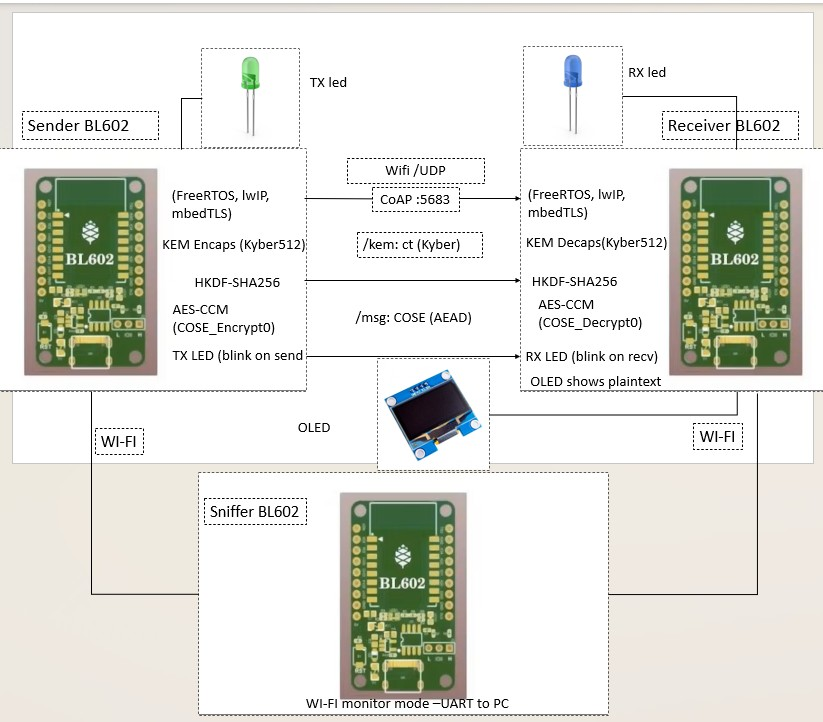
\includegraphics[width=\columnwidth,height=8cm,keepaspectratio]{IOT (2).jpg}
\caption{System architecture.}
\label{fig:system_arch}
\end{figure}


   \begin{figure}[H]
  \centering
  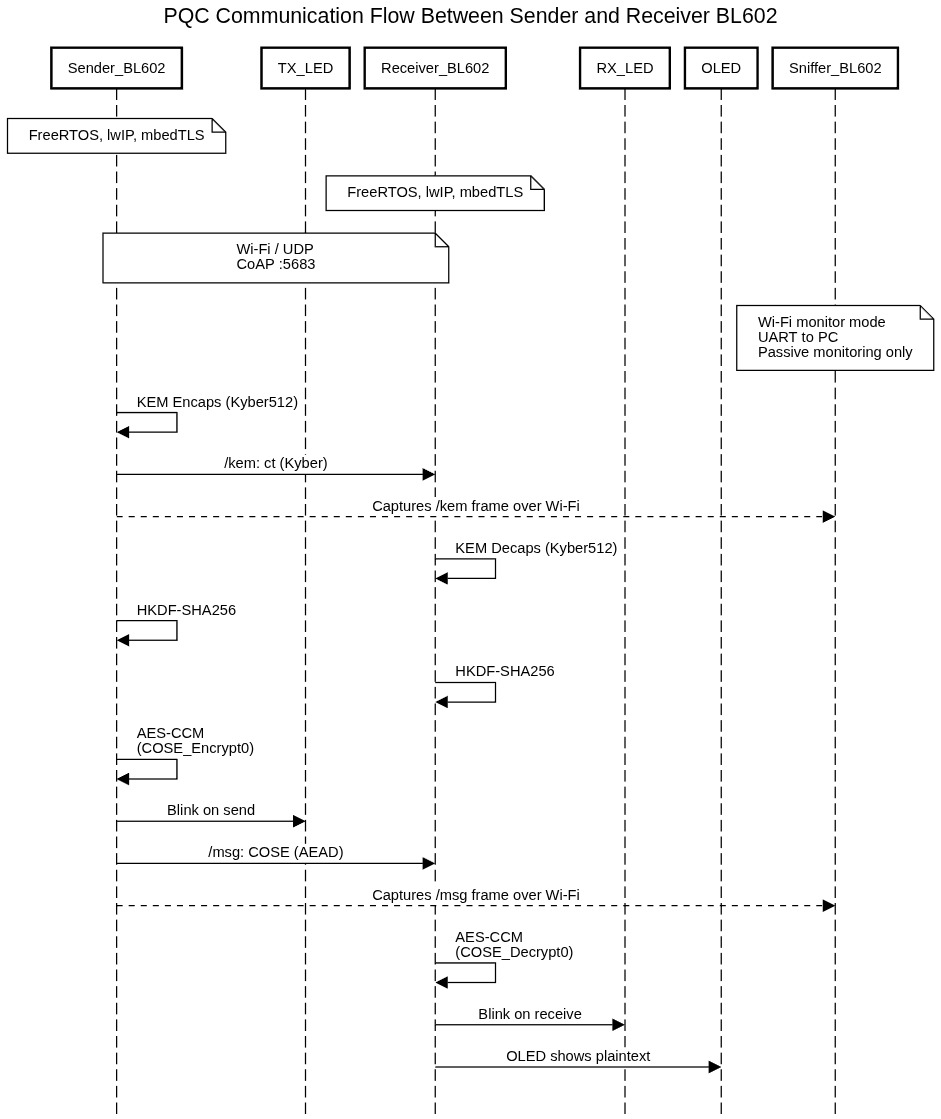
\includegraphics[width=\columnwidth]{uml.jpeg}
  \caption{Sequence Diagram.}
  \label{fig:seq_diag}
\end{figure}

\begin{figure}[H]
\centering
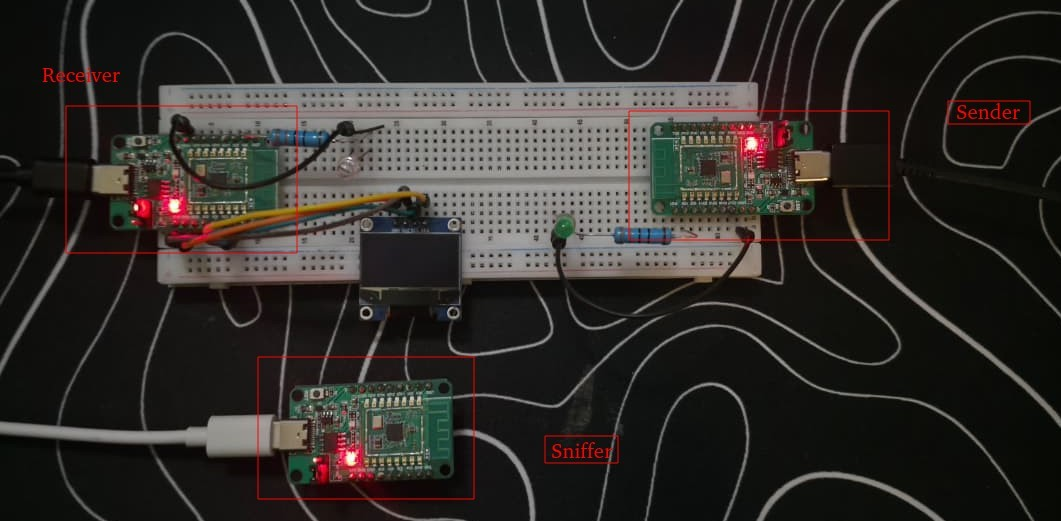
\includegraphics[width=\textwidth,height=0.45\textheight,keepaspectratio]{prototype.jpg.jpeg}
\caption{System Prototype}
\label{fig:sys-prototype}
\end{figure}

    \subsection{Software Development}
    Initially, the use of the BL602 microcontrollers enables firmware development for a limited firmware stack for each of the PineCone boards (the Sender board, Gateway board, and Sniffer board) that allows CoAP-over-UDP communication to be performed in a secure manner. Each of the three boards uses the C/C++ programming language and is developed with the use of the BL602 SDK. Each of the firmware applications runs on FreeRTOS (a small real-time operating system) and has a network stack named lwIP.

    The three PineCone boards all share a common start-up pattern based on FreeRTOS and the use of lwIP:

    \begin{enumerate}
    \item System Initialization:  Each node, when the reset occurs will execute its microcontroller core system initialisation such as clock and memory, uart, led gpio pins.
    \item Wi-Fi Connection: A Wi-Fi specific, process is charged with the responsibility of configuring the radio to act as a station, connect to the access point with pre-programmed credentials and wait to receive the response of DHCP, i.e., giving the node an IPv4 address. Once the node has received its IPv4 address, the Wi-Fi-specific task will print the networking information to the serial console and then set a global flag indicating that the node is now ready to communicate over the network.
    \item Application Start-up: Once the global flag indicating that the node is network-ready has been set by the Wi-Fi task, an application-specific task will wait until the global flag is set and then, when the flag is set, will begin executing the proper logic associated with the Sender board (Sender), Gateway board (Gateway) or Sniffer board (Sniffer).

    \end{enumerate}

    \subsection{Implementation}
    Once initialized, each PineCone (BL602) begins executing an application task depending on its specific role:
    \begin{enumerate}
    
    \item PineCone(gateway):
    
    \begin{itemize}
    \item It holds a long term ML-KEM-512 keypair in flash memory and provides the Sender with the public key.
    \item Listens for CoAP requests on UDP.
    \item Decapsulates using ML-KEM, calculates the AEAD key with HKDF-SHA-256, then decrypts or verifies AES
    \item Prints the decrypted message to the local OLED screen.
    \end{itemize}

    \item PineCone(sender):

    \begin{itemize}
        \item It uses the Gateway public key for the ML-KEM-512 encapsulation procedure to derive the shared secret.

        \item Performs the HKDF-SHA-256 function to derive the 128-bit AES

        \item Creates a minimal CoAP over UDP message, then encrypts/authenticates the message using AES-CCM

        \item Rejects Duplicates/unexpected messages with freshness rules

    \end{itemize}

    \item PineCone(sniffer)

    \begin{itemize}
        \item Runs in Wi-Fi monitor mode to capture IEEE 802.11 frames that are nearby.
        
        \item Streams the frames over UART/serial to a host-side decoding script

        \item This is then decoded for analysis in Wireshark to look for any anomalies.The Sniffer PineCone sends the captured 802.11 frame data to a host computer through the serial connection. A small decoding script on the host computer translates the captured data into a form that can be opened as a capture interface. This means that the data can then be captured and filtered in real-time using Wireshark while the application data is encrypted with AES-CCM. 
    \end{itemize}

    \end{enumerate}

     

    \section{Threat Model and Security Testing}
    \subsection{Attacker Model}
    For the purpose of this project, it is assumed that the Attacker is on the same local Wi-Fi or Local Area Network (LAN) as the Sender and Gateway Devices. As most IoT devices exist on the same Wi-Fi/LAN network, this is considered to be a very realistic/common threat vector associated with IoT Devices. Many IoT devices are found on a number of different Networks (e.g., Home Network, College Network, Office Network, etc. ), and an Attacker can also be found on the same Network. Because of this Reality, the Attacker does NOT need Physical Access to either the Sender or Gateway Device in order to perform his attack. In other words, the Attacker possesses Network/Internet-based capabilities such as Scanning or Device Placement for the purpose of executing Attacks. Finally, the Attacker sees ALL Network Traffic between the Sender and Gateway at the level of IP or UDP, and can also execute other forms of attack in addition to the IP or UDP level attacks. This threat model aims to verify that the project’s security is robust against an attack considering an attacker will have full visibility over the network traffic. However, as mentioned previously in the chapter, although the attacker has full visibility of the network traffic, they do not have access to cryptographic secrets that are stored on the Gateway device.

    \subsection{MITM / Sniffing Observation}
    In order to see how the security of network breaches is compromised, a set of packet captures was performed from the perspective of the attacker (using Wireshark). The MITM enabled the attacker to see, just as a legitimate user does, that there was communication taking place and was able to obtain information about each message. This information includes sender IP address, receiver IP address, UDP port number used for the CoAP message (CoAP uses default port 5683), size of each packet transmitted, order that packets are being transmitted in, type of request being sent over CoAP message (type is POST), etc. However, the most significant piece of information that the attacker could see was that the payload of the /pqkem-data message contained random values of bytes. This random value in the payload indicates that there is no text based data within that payload; instead, it contains post-quantum KEM ciphertext (encrypted) data, an AEAD nonce, AEAD ciphertext and an AEAD authentication tag.The attacker has access to the bytes of the packets they have seen; however, they will be unable to decipher the meaning of those bytes due to the fact that the key that deciphers the message was never transmitted. The key for AEAD encryption is derived from the shared secret generated by MLKEM; however, in order to decapsulate the shared secret requires knowledge of the Gateway's private key, which is only stored in the Gateway itself. Therefore, from the perspective of the attacker, knowing the packets exist and that some communication is happening on the network provides evidence that the data and/or packets do, in fact, comply with the principle of "secure even when the network has been compromised." A screenshot of Wireshark showing CoAP packets and the ciphertext in the payload will serve as [Figure 6 and 7] to support this statement.
    \begin{figure}[H]
  \centering
  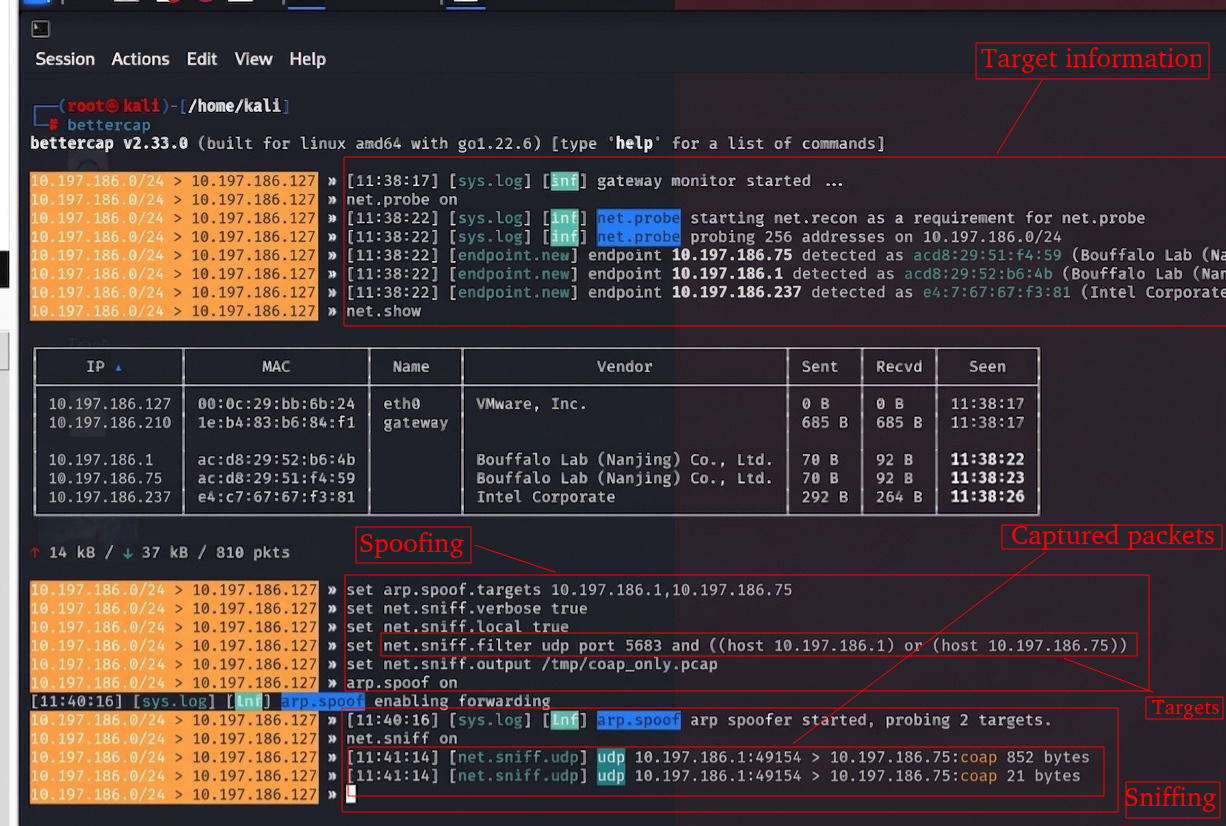
\includegraphics[width=\columnwidth]{Arp spoffing.jpeg}
  \caption{Arp Poisoning}
  \label{fig:arp-spoof}
\end{figure}

\begin{figure}[H]
\centering
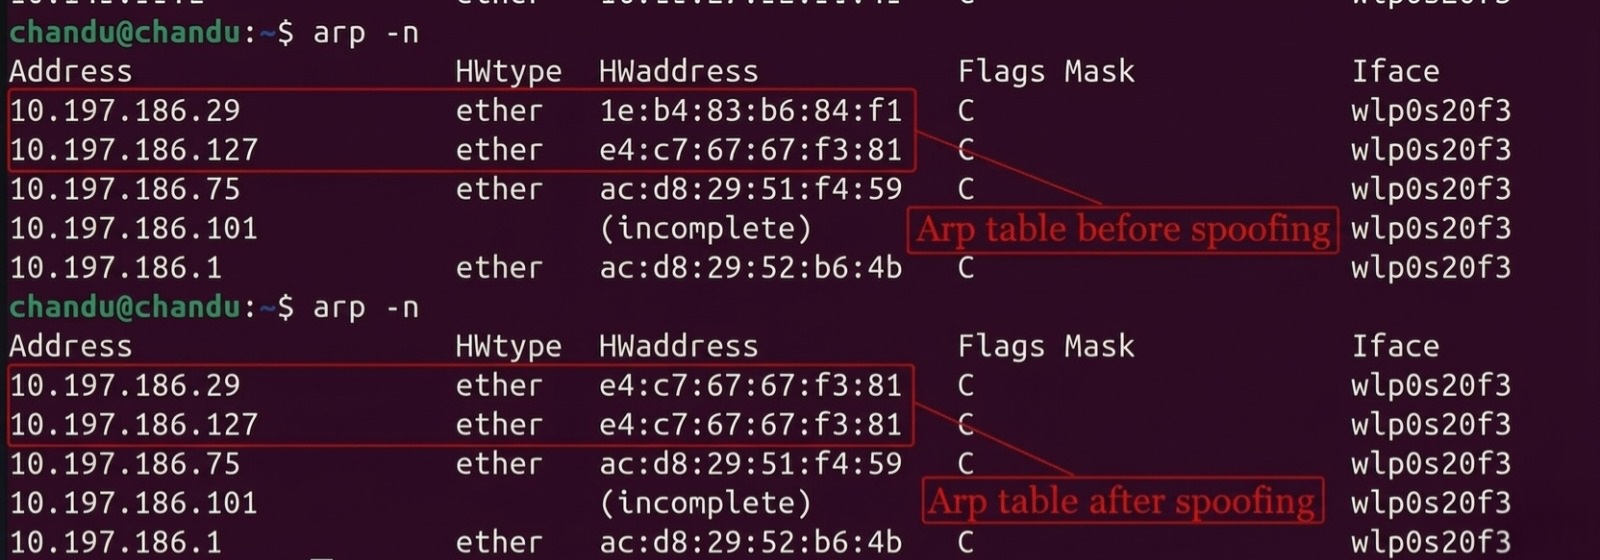
\includegraphics[width=\textwidth,height=0.45\textheight,keepaspectratio]{Arp_Table.jpeg}
\caption{ARP Table}
\label{fig:arp-table}
\end{figure}

\begin{figure}[H]
\centering
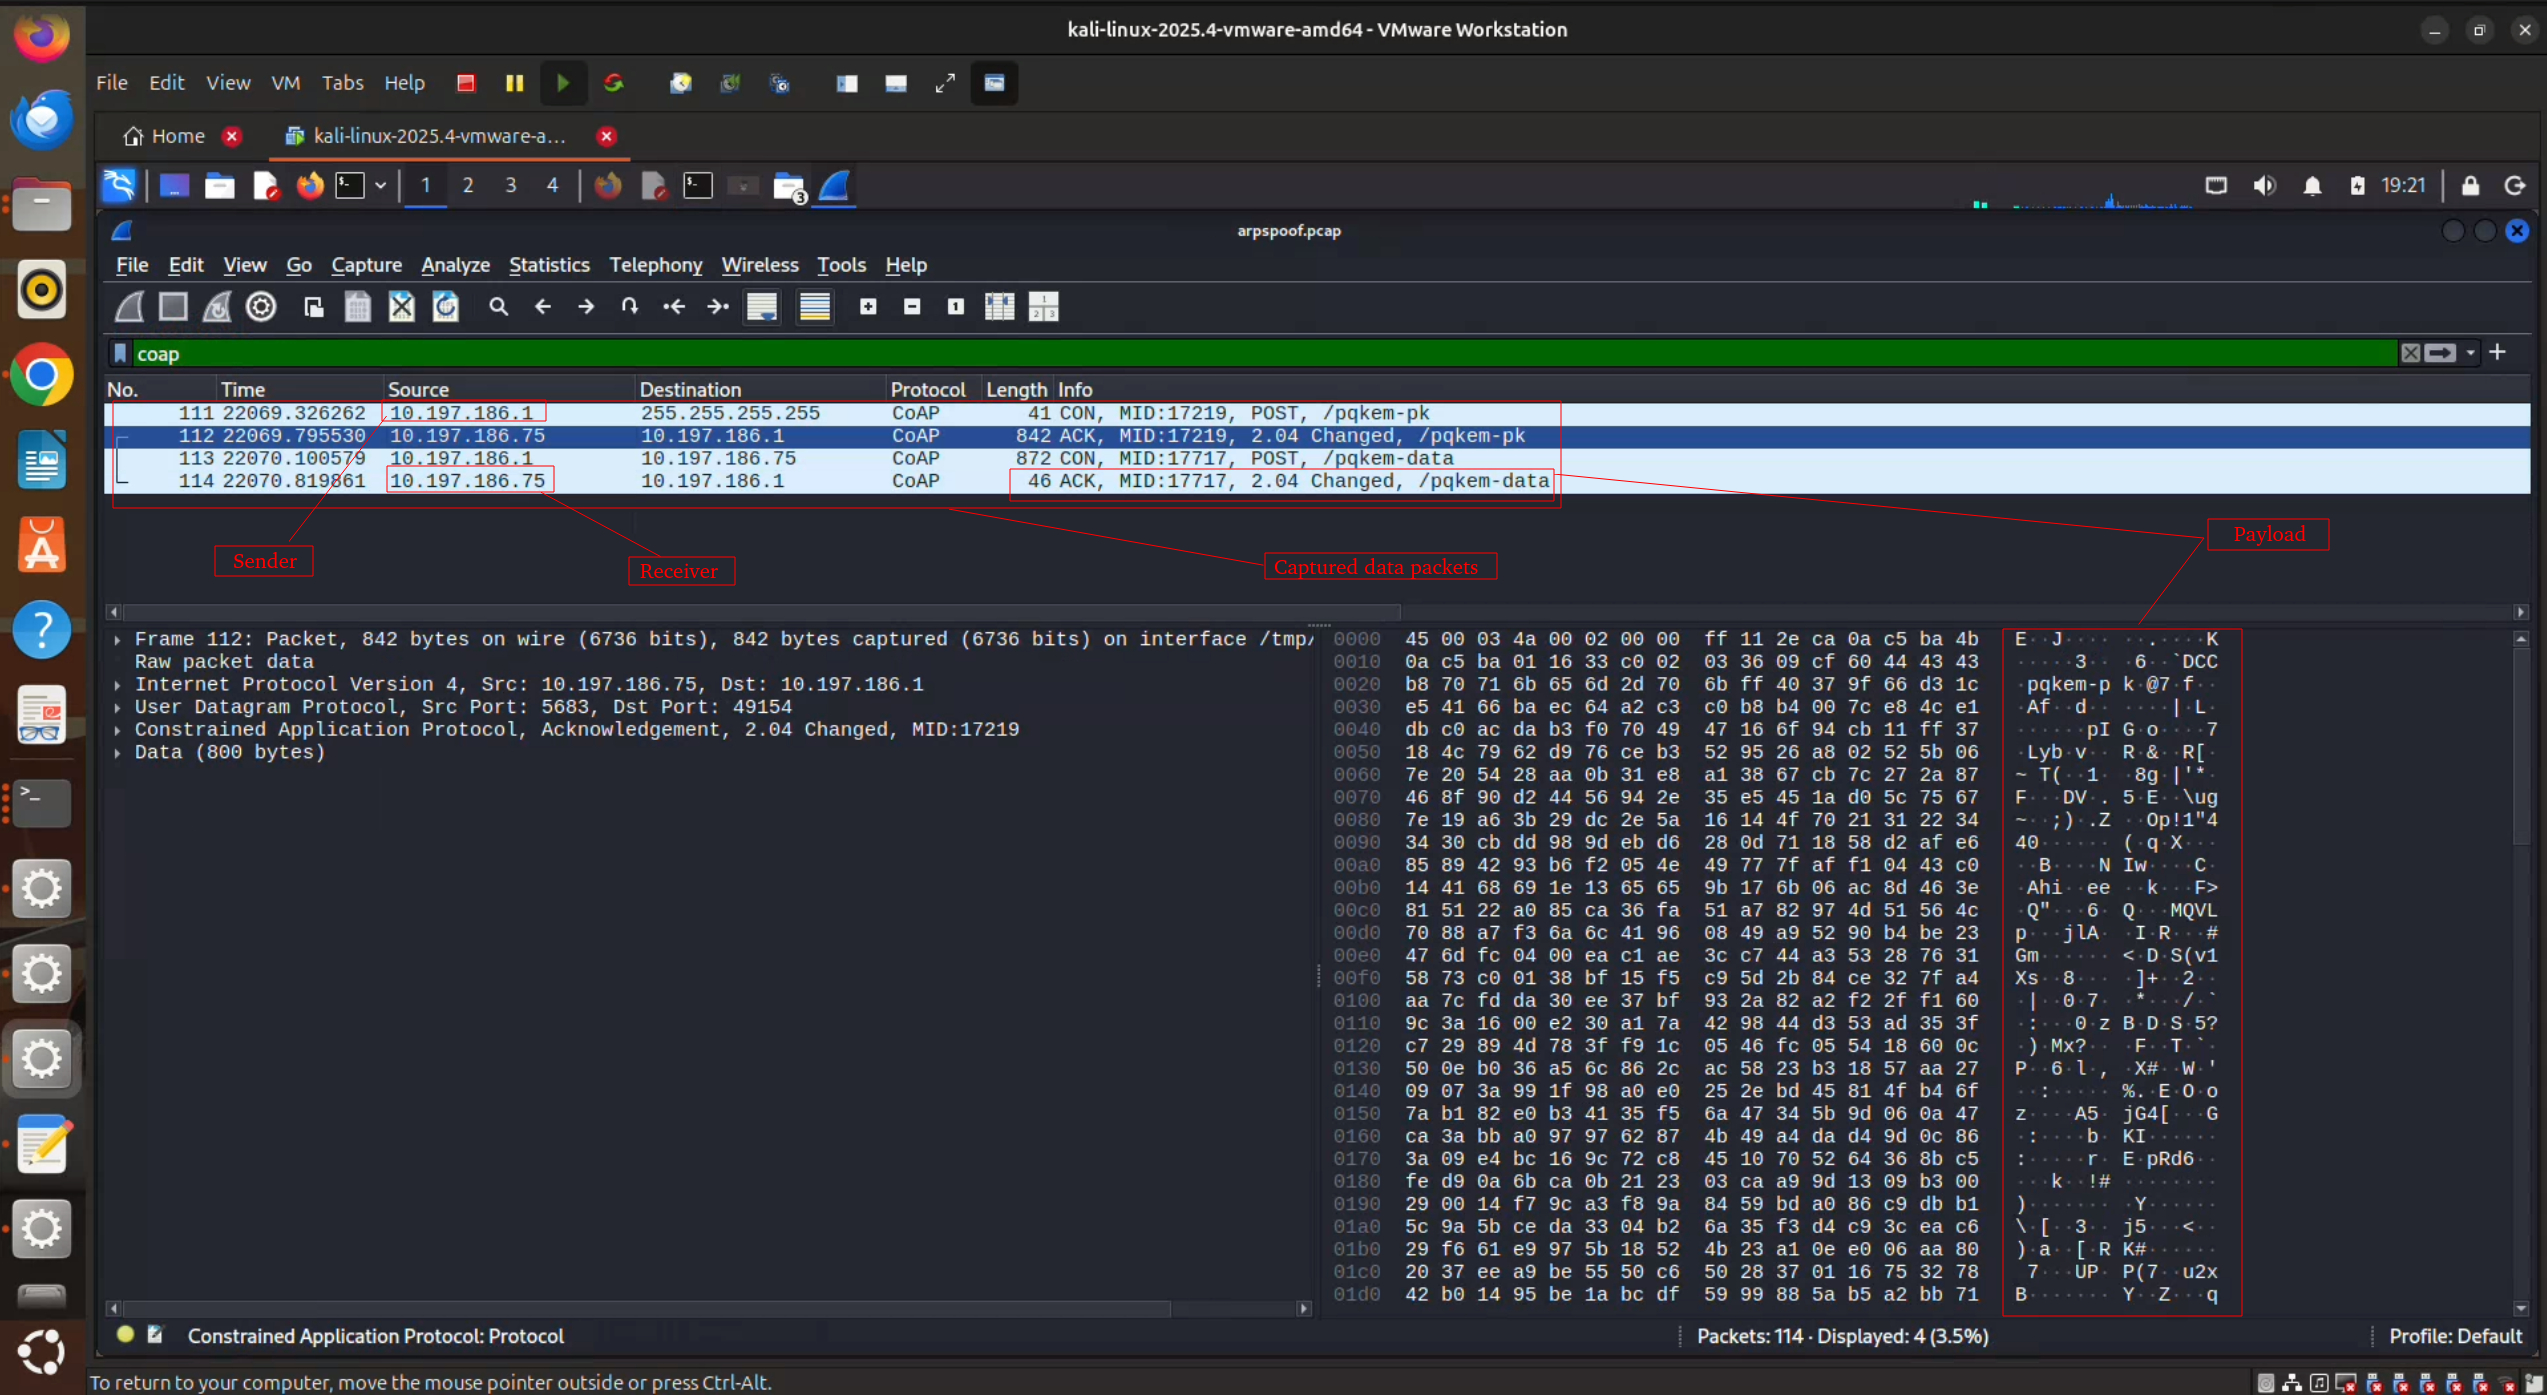
\includegraphics[width=\textwidth,height=0.45\textheight,keepaspectratio]{data packets.jpg.jpeg}
\caption{Data packets captured by the attacker}
\label{fig:data-captured}
\end{figure}

To evaluate the capability of the attacker to observe the messages transmitted using a transmission, an interception test was completed by ARP spoofing the transmission to intercept the data while using Wireshark to create a record of the network traffic.Using an ARP Poisoning filter to review the captured packets, it was determined that although the attacker could successfully intercept and view the CoAP packets, the actual content of the CoAP messages was still secure. The attacker could not read the plaintext because the payload was successfully protected as encrypted ciphertext.

\begin{figure}[H]
  \centering
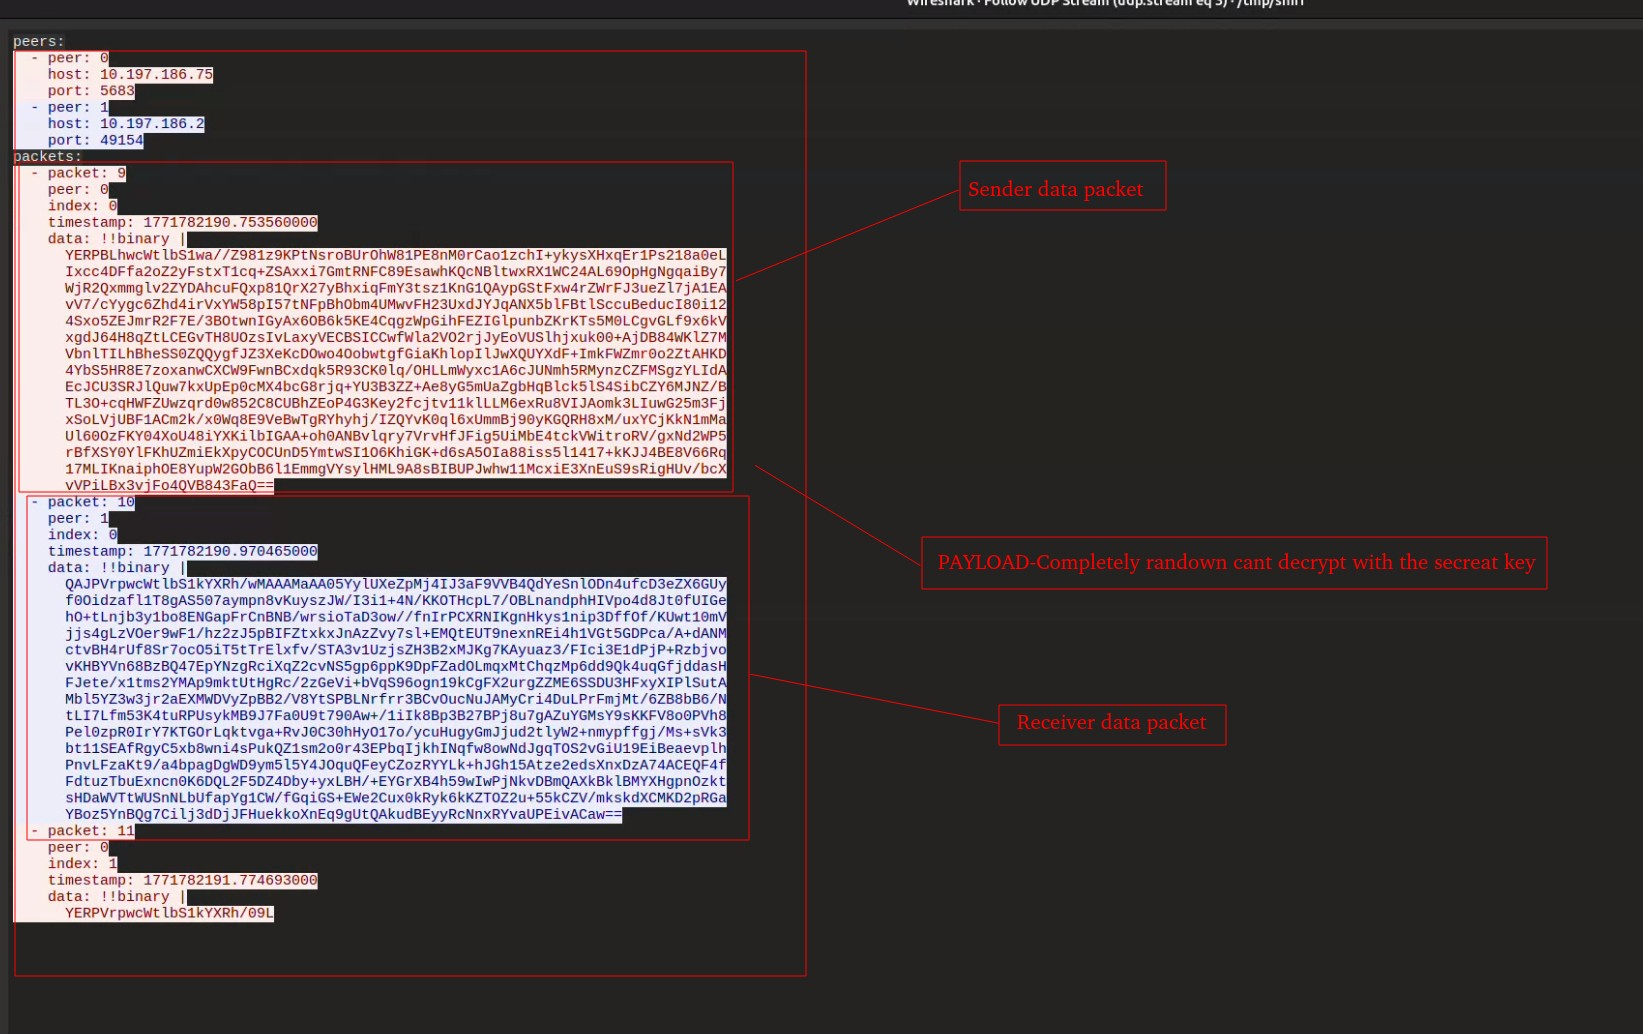
\includegraphics[width=\columnwidth,height=7.5cm,keepaspectratio]{Payload.jpg.jpeg}
  \caption{Packet Payload}
  \label{fig:payload}
\end{figure}


    \subsection{Tampering Detection}
    Apart from confidentiality, the communication also needs to ensure integrity, which means that the attacker must not have the capability to alter the communication without being detected. For testing this requirement, the project also includes the controlled tamper simulation, which flips one bit or byte of the protected payload after encryption, i.e., after AES CCM has generated the ciphertext and the authentication tag. This simulation is based on the assumption that the attacker may intercept the communication packet and alter some of the bytes. AES CCM is an AEAD mode, which stands for Authenticated Encryption with Associated Data. Therefore, AES CCM encrypts the communication as well as authenticates the communication. While decrypting the communication, the Gateway also recomputes the authentication tag. If the communication packet, the authentication tag, the nonce, etc., have been altered, the authentication tag does not match. Therefore, the Gateway does not output the plaintext. Instead, the Gateway rejects the communication packet and prints the message “AEAD AUTH FAIL” or “Decrypt FAIL” on the OLED. Therefore, the Gateway’s behavior in this case is also an important security proof, which shows that the communication cannot be tampered with, even if the attacker can intercept the communication packet. 

    \begin{figure}[H]
  \centering
  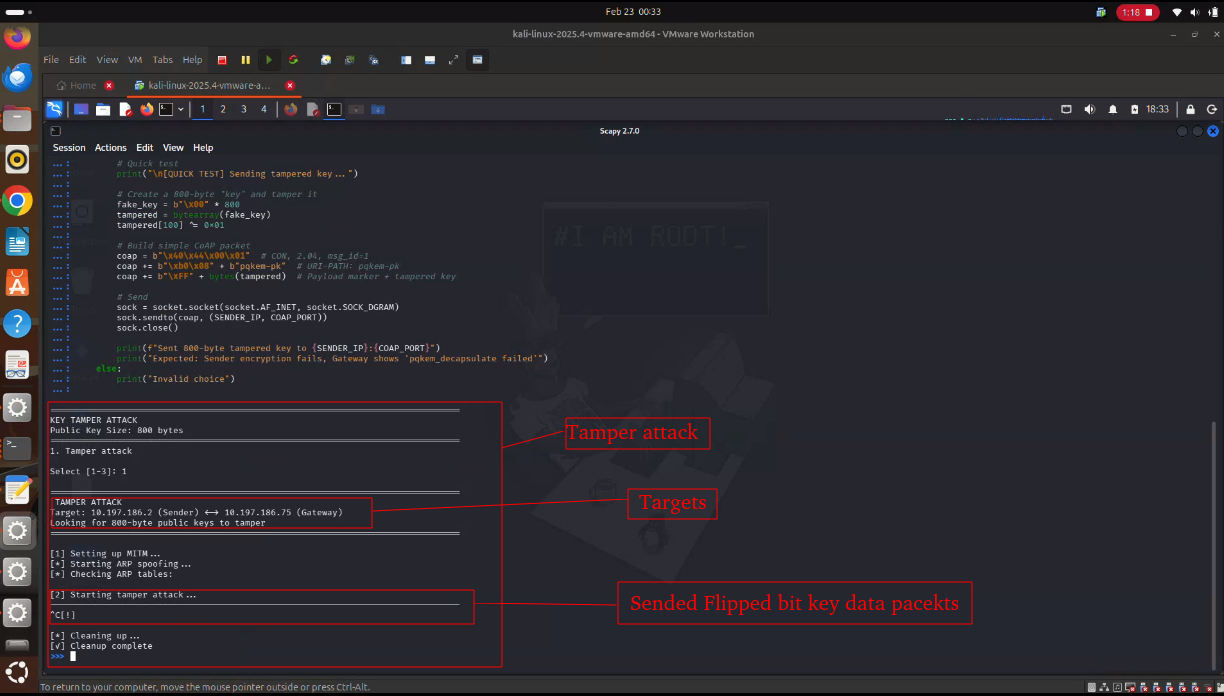
\includegraphics[width=\columnwidth]{tamper attack.jpg.jpeg}
  \caption{Tamper Attack}
  \label{fig:tamper-attack}
\end{figure}

\begin{figure}[H]
  \centering
  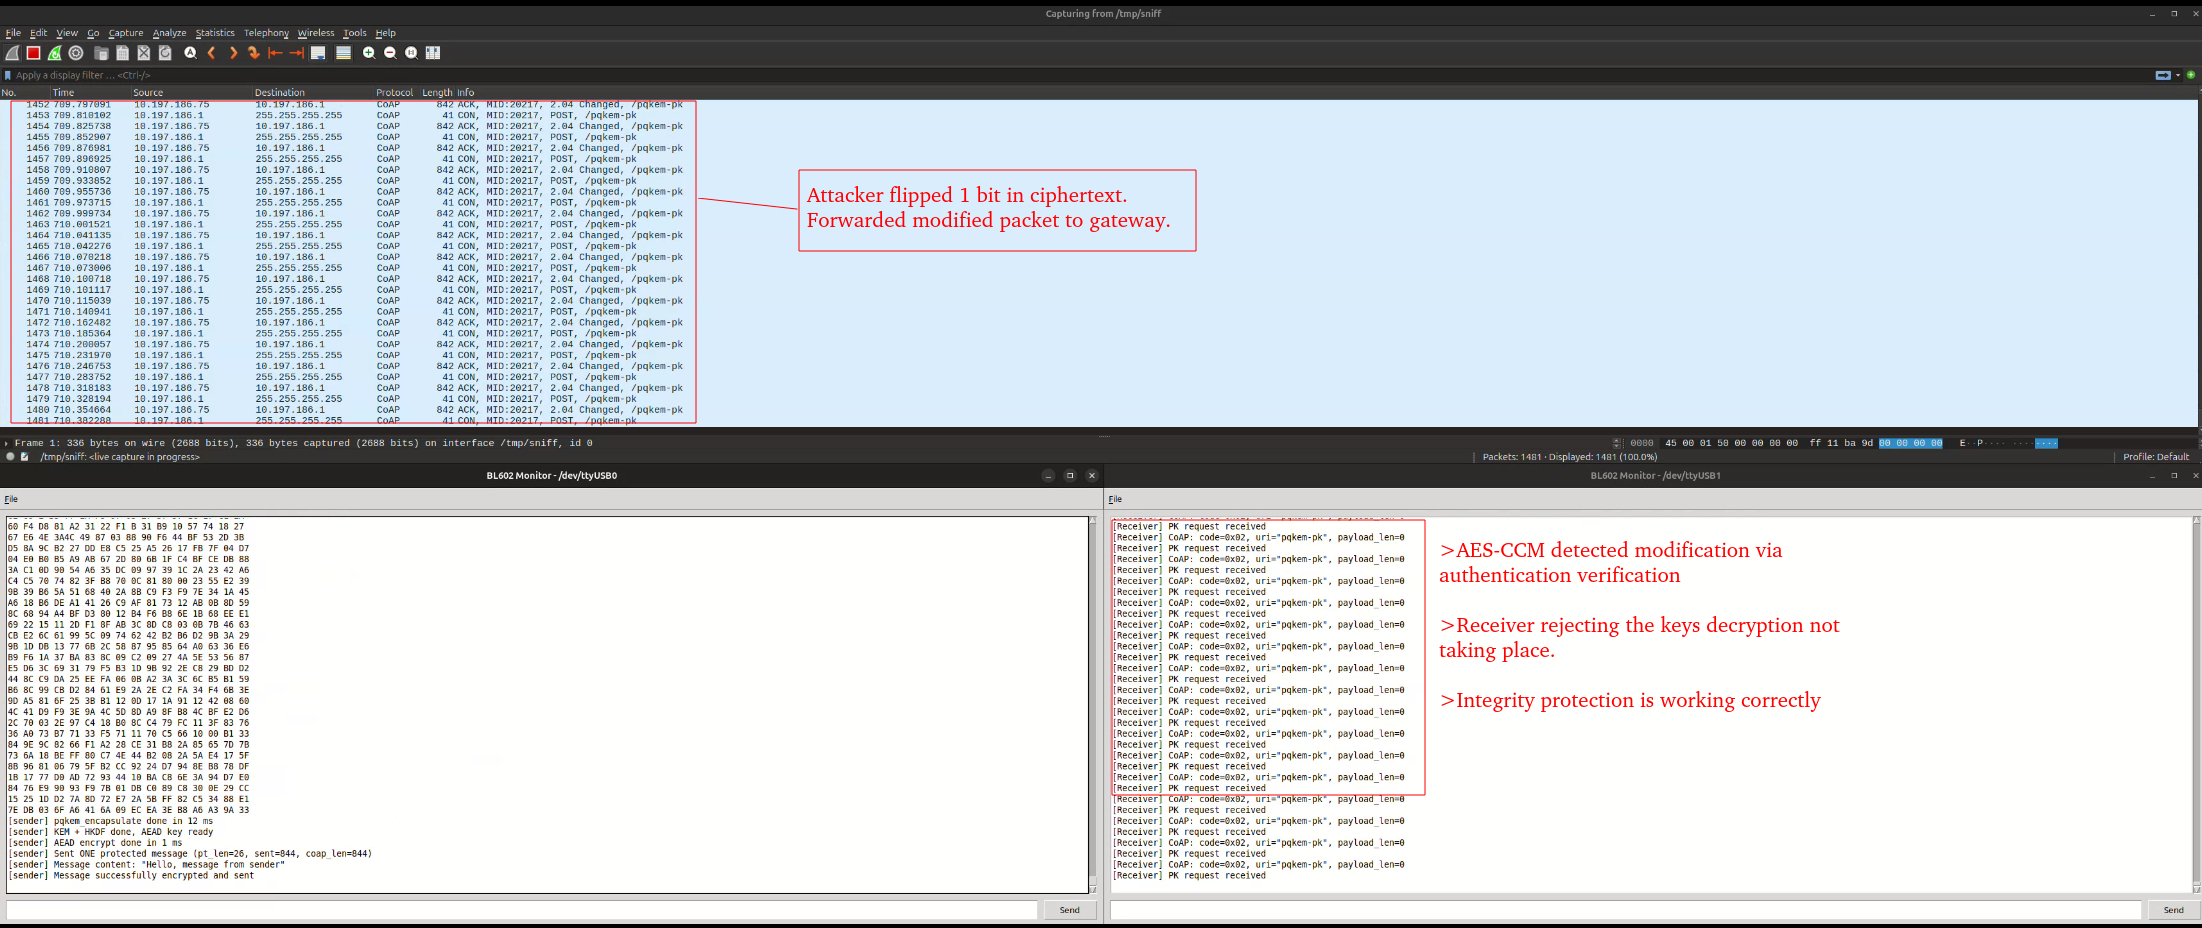
\includegraphics[width=\columnwidth]{Tamper attack result.jpg.jpeg}
  \caption{Tamper attack result}
  \label{fig:tamper-result}
\end{figure}

     \section{Security Analysis and Validation}
     
        \subsection{Security Properties Verified}
        Our security tests will confirm that our security measures satisfy the following security properties that industries require from secure communication systems: First, even when the attacker receives the packets sent from the communication system, the payload will still be encrypted, ensuring the confidentiality of the information. Secondly, when the attacker alters any part of the encrypted message, the gateway will be able to identify the alteration since the authenticated encryption will fail to pass the verification. Lastly, the attacker will not be able to compromise the security of the communication system even when positioned in the middle since the security measures do not rely on “trusted routing.”

        \subsection{Why This System is Secure}
        This system employs post-quantum key establishment and authorised encryption systems built-out correctly and structured; both contribute to its secure nature. By utilizing ML-KEM-512, the expectation is that the session secrets cannot be easily inventoried by quantum computers in the same way as classical methods. After establishing POST-QUANTUM keys, both parties will run HKDF-SHA256 to derive AES keys from their respective keying material; this process ensures the deriviation of keying materials is uniform, consistent across both parties and application specific vs. using derived keys based on their raw materials. The AES-CCM algorithm will be used to encrypt/authenticate the payload, creating confidentiality and integrity for each message transmission as both will be guaranteed security regardless if the attacker can see the traffic or try to disarm the message being transmitted. While an attacker may be able see any individual piece of traffic; they will not be able to decrypt or alter the transmission without detection. In addition, using nonces allows the receiving end to verify that an incoming nonce has not been previously received; therefore, discarding any older nonce-based command packets to prevent re-execution of prior commands.

        \subsection{Security Features in the Project}
        The Primary Security Implementation within this project is Post-Quantum Key Exchange via ML-KEM. In the process flow, the Provider will request the Gateway Public Key, and then the encoder will generate KEM ciphertext together with a Share Secret when generating the KEM ciphertext. The KEM ciphertext can be safely transmitted while the One Time Key is kept Private. The only Person who can access the One Time Key (OTK) is the Gateway, as he holds the Matching Private Key, thus able to Decrypt/Decapsulate the KEM ciphertext and retrieve the One Time Key. Therefore, if an Attacker were to succeed in obtaining the KEM ciphertext, they would be unable to Calculate/Derive the One Time Key therefore would not be able to obtain the Symmetric Encryption Key.

        The next Major Security Implementation within this project is key derivation using the HKDF-SHA256 Algorithm instead of using the KEM shared secrets symmetric key. The project uses HKDF to derive a session key using a fixed "info" Context String (i.e., "ML-KEM-AEAD"). These steps will prevent the Generation of Weak or structure KEM-derived session keys and ensure that the session key will be securely aligned and Common to both ends of the AES-CCM communication.

        In this project, we are implementing the third security feature to ensure that messages sent from the device are safe to receive. To accomplish this task, we are using the AES-128-CCM algorithm. The combination of the attribute of the authentication tag and the ciphertext will allow you to know who did send the message and its contents. If an attacker attempts to modify the message by altering the ciphertext by even one bit, the gateway will know immediately and will reject the message. This is what is happening when the "AUTH FAIL" and "Decrypt FAIL" messages display during the tamper test. This is critical to our project because we do not want to give an attacker the ability to modify commands to the device and change the physical processes controlled by the device.

        \subsection{Monitoring, Detection, and Practical Security Measures}
        Real-time features of your project offer very clear indicators of security incidents that can be monitored easily. For example, if a user attempts to authenticate multiple times unsuccessfully this may indicate that someone is trying to tamper with their packets. In the industrial environment these events could then be sent to a log server or SOC monitoring tool for take appropriate action in response. The ability to validate the cryptography of your project makes it a strong security measure since the encrypted data represents the first barrier to prevent someone from committing an attack, while the above examples of failed authentication attempts represent the second barrier.

        While ARP spoofing attacks, which are a type of man-in-the-middle attack, might be able to reveal the contents of network traffic between two parties, they do not break cryptography; rather, they provide an attacker with the ability to observe and relay communications between those two parties. Your project is still secure from the attacker because he does not have access to the post-quantum shared secret or to the AEAD key derived from that secret. The attacker is only able to affect communication in two ways: by reducing the visibility of those communications (by dropping packets) or by reducing the validity of those communications (by altering the contents of those communications, thus causing the recipient to reject them during authentication). Therefore, the total security of the system is entirely dependent upon the successful implementation of cryptography and has nothing at all to do with having a trustworthy network.

    \section{Industry Usefulness and Real-Time Impact}
    This model is directly applicable to the real world due to the fact that most IIoT networks assume that the network cannot be trusted. In most industries, devices will communicate with each other over a shared Wi-Fi/LAN network. In such a network, the attacker could potentially connect to the same network as the devices and sniff the network to gain information from the devices. This is exactly what your project demonstrates: security is not dependent on the router/Wi-Fi network being “safe,” but on the security that is implemented within the devices. This is similar to the “zero trust” model that is currently being implemented within the industry. This model will protect the devices even in the event that the network is compromised. In most industries, devices will last for a long time—5 to 15 years. In such a case, the fact that your project utilizes a post-quantum ML-KEM is beneficial to the security of the devices.
    The most critical aspect of IIoT networks is preventing attackers from interpreting sensor information that has been sent to a controller. Your project accomplishes this because it prevents the attacker from interpreting sensor information sent to the controller. Likewise, the attacker will be unable to send any information to the controller. As a result, the receiving device will know that the received information is an attempt at tampering. With respect to operation, the security messages (e.g., AUTH FAIL) that the gateway will send could be employed in a way that directly applies to physical businesses because the same security messages could be used with the various security monitoring systems deployed in different manufacturing facilities.

    \section{Challenges,Resolution and Outcomes}
    \subsection{Challenges we faced:}
    The solution implementation and evaluation had challenge issues which are common in embedded system IoT security prototyping. The greatest problem was to ensure that there was successful packet-level observability when communicating between the sender and the gateway. This proved to be such a challenge because packet capture is not always effective on the Wi-Fi network when there was effective communication between the gateway and sender because of a range of VM network limitations, interface mis-selection, access point interaction in the network and capture filter settings which may obscure CoAP/UDP packets over short periods. Conversely, the interpreting network addressing and routing was the second problem in implementing and assessing the solution. The third challenge that caused this to be a challenge was the aspect of relating to tooling and stability of the build in the implementation and evaluation of the solution whereby even though the log indicated that the data was sent, the communications were lost at the application level. The component tree had build dependencies missing, as well as problems with script execution permission controls, use of non-UTF8 serial output, which, possibly, interacted with monitoring tools.

    \subsection{How we resolved:}
    To address mitigation and resolution of workflow and implementation challenges, the project provided repeatable and defendable evidence for project evaluation by implementing a deterministic packet capture workflow rather than relying on the passive sniffing of third devices in dynamic wifi environments. In efforts to resolve network configuration issues, the project implemented proper destination addressing by forcing endpoint CoAP messages to be sent to the designated IP address of the gateway board's IP address with the associated router/AP acting only as a strict forwarding device in lieu of application endpoints. The project also incorporated tooling hardiness by utilizing a tolerant serial decoding process that allowed valid packet marker identification to occur even when the serial data was made up of non-text binary digits. Additional examples of resolution of build and execution challenges use reconfiguration of the components, by removing unused dependencies and/or adding missing source codes, correcting permissions on the scripts, and standardizing the methodologies of flashing and selecting ports for building, flashing, and running, to ensure that the process of building, flashing, and executing are performed in the same manner consistently.

    \subsection{Outcomes:}
    The project contributed a lot to the learning and knowledge acquisition of the project team on cryptography and embedded systems engineering. Security wise, the project enhanced the understanding of the project team on the operation of a KEM-KDF-AEAD pipeline. The project showed that a symmetric key could be safely generated and exchanged between two endpoints by the ML-KEM key exchange. The project has shown how it is possible to generate a secure symmetric key using the HKDF-SHA-256 key derivation function and then use it in the authentication and encryption process. Through the AES-CCM encryption and authentication system, the project provided an indication of how a symmetric key could be used to guarantee the confidentiality and integrity of the data that is being sent between points, whereby modification of the data would provide a certain failure of authentication. The engineering and evaluation sides, the project enhanced the project team knowledge on how to assess and report the project outcome, whereby, the relevance of packet sniffing and sensitivity of packet sniffing to the network architecture and the tools in use were proved. Lastly, the project enhanced the knowledge of the project team concerning the significance of dependency hygiene, proper logging, proper script permissions and clean build processes because these are significant towards project validation and presentation of project results.

    
    \section{Evaluation and Results}
    \subsection{Functional Behaviour}
    The system was consistent across the repeated runs. The reset made both Sender and Gateway the Wi-Fi network members, where they received IP addresses through DHCP and displayed them in the serial console. After the network was prepared the Sender sent a CoAP request to the public-key resource of the Gateway and received as always a response whose payload length corresponded to the ML-KEM-512 public key.With this key, the Sender then transmitted a second CoAP POST which took the ML-KEM ciphertext along with the AES-CCM encrypted payload. According to the logs of the Gateway, CoAP was correctly parsing, after which there was a successful decapsulation and decryption. The plaintext that was recovered was also displayed on the serial console and on the OLED display, thus verifying that the message content is only learned by the Gateway. LEDs on the Sender and Gateway would momentarily flash on every successful run. On the whole, these observations demonstrate that CoAP, ML-KEM, AES-CCM and persistent key storage are collaborative as a full-fledged end-to-end system.
    \subsection{Performance Measurements}
    Cryptography routines were embedded in a timer that had a timing resolution of milliseconds. The ML-KEM-512 decapsulation processing on the gateway had a time requirement of approximately 11 to 12ms (same as the time required for ML-KEM-512 encapsulation). Based on the measured values of the short status message used in the demonstration, the processing of AES-CCM Encryption and Decryption all completed under 1ms and effectively fell below the resolution of the timer; therefore, obviously, the post-quantum overhead is the primary factor in the timing. The latency timing values will be acceptable within the common latency budgets for IoT devices and applications. A single delay of several ten milliseconds for a one-time configuration of a session is marginal compared to typical network and application delay. The memory used was within the normal limit of the capabilities of the boards. The ciphertexts and keys are stored in static buffers, while the payload for CoAP security will be stored in easily accessible RAM. Because the application is non-dynamic, it will be considerably easier to estimate resource consumption in the worst-case scenario.

    \begin{table}[H]
\centering
\begin{tabular}{|l|r|p{7cm}|}
\hline
\textbf{Parameter} & \textbf{Result} & \textbf{Meaning} \\
\hline
ML-KEM-512 encapsulation time & $\sim$11--12 ms & Time taken by sender to generate shared secret and ciphertext \\
\hline
ML-KEM-512 decapsulation time & $\sim$11--12 ms & Time taken by gateway to recover the shared secret \\
\hline
AES-CCM encryption time & $<$ 1 ms & Time taken to encrypt the message \\
\hline
AES-CCM decryption time & $<$ 1 ms & Time taken to decrypt the message \\
\hline
Public key size & 800 bytes & Size of gateway public key sent to sender \\
\hline
Ciphertext size & 768 bytes & Size of ML-KEM ciphertext sent in secure data message \\
\hline
Shared secret size & 32 bytes & Secret used to derive AES session key \\
\hline
\end{tabular}
\caption{Performance and size metrics of the implemented cryptographic system}
\label{tab:crypto_results}
\end{table}

\begin{table}[H]
\centering
\begin{tabular}{|l|r|p{7cm}|}
\hline
\textbf{Parameter} & \textbf{Result} & \textbf{Meaning} \\
\hline
Flash-backed firmware size & 615,598 bytes & Memory occupied by program code and read-only data \\
\hline
Final binary size & 615,724 bytes & Size of generated gateway firmware file \\
\hline
Static RAM-backed memory & 109,092 bytes & Total fixed RAM reserved by the gateway build \\
\hline
UDP receive buffer & 1,024 bytes & Buffer used to receive CoAP packets \\
\hline
Key storage structure & 2,440 bytes & Space used to store gateway post-quantum key material \\
\hline
\end{tabular}
\caption{Memory usage statistics of the gateway firmware}
\label{tab:memory_usage}
\end{table}


    
    \subsection{Packet level analysis}
    The Sniffer node captured traces which were then viewed in Wireshark and provided a network-level overview of the overall system. In the packet captures we see ARP and DHCP traffic as such traffic occurs when the board connects to the network. A subsequent CoAP POST message containing the public key was sent from the sender to the gateway, WS displays CoAP headers and the data itself as a block equal to the size of the public key. Subsequent data messages were sent using a different larger CoAP POST message, the payloads travelled as ML-KEM encrypted ciphertexts of 768 bytes in size along with AES-CCM nonce, the encrypted data and tag. CoAP has complete decoding capabilities for all of its header types and only the payload consists of random bytes created from proper application of encryption of the activity on the network. Synchronizing this with LED flashes and serial data, along with OLED information, will allow for correlation between what is being performed by the device and what you see on the wireless link.

     \begin{figure}[H]
  \centering
  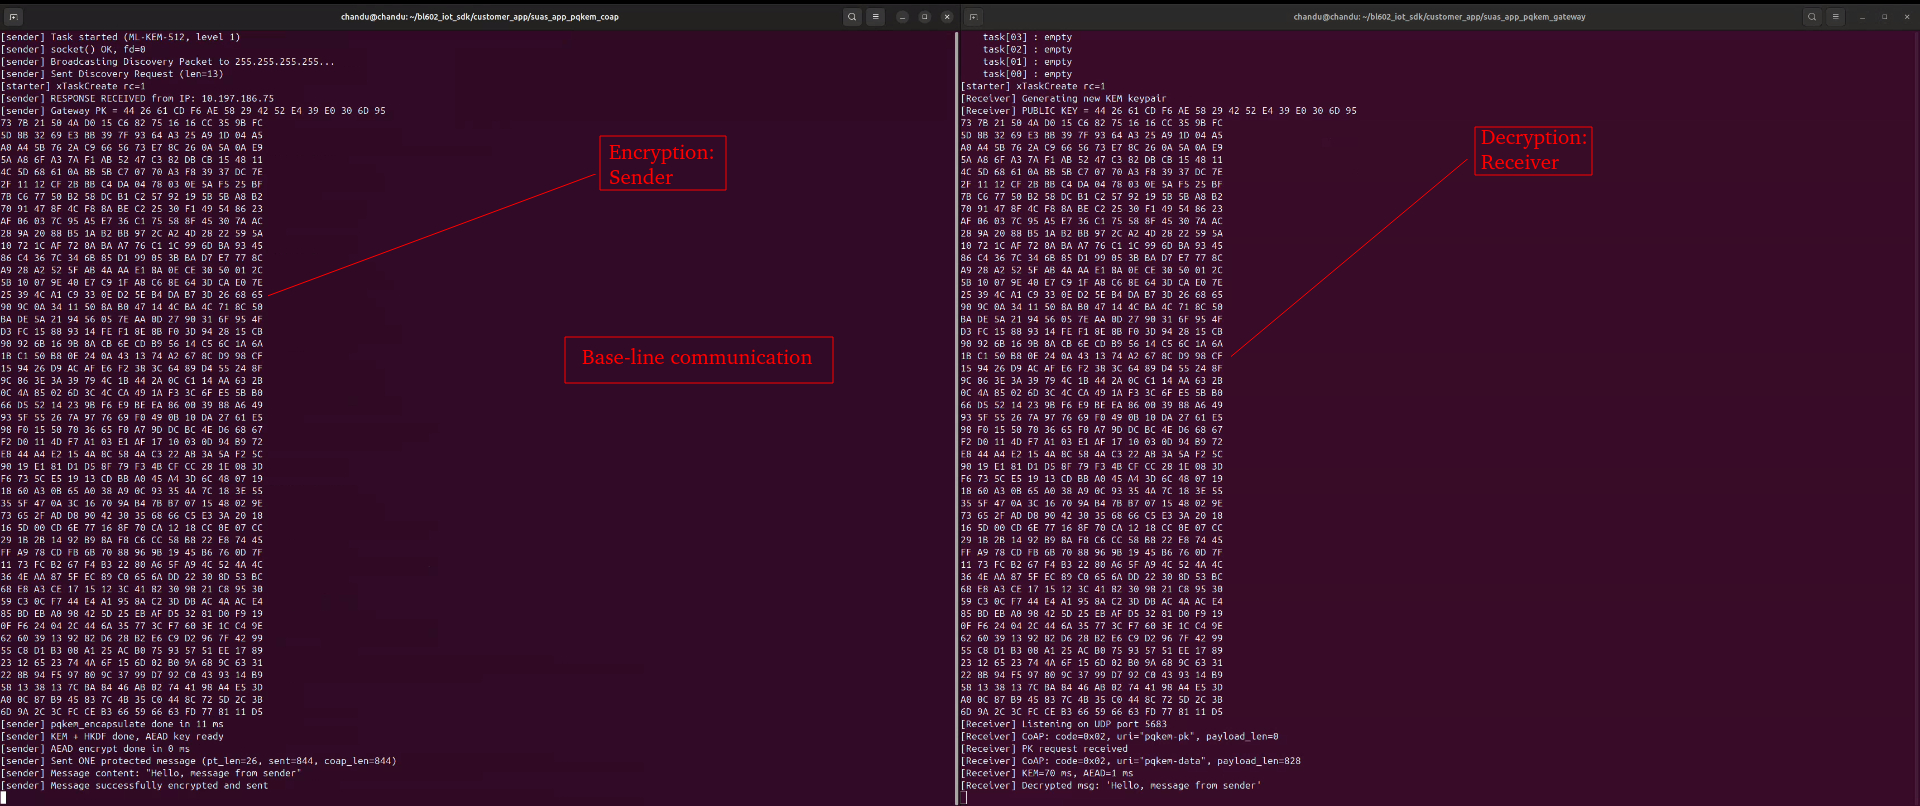
\includegraphics[width=\columnwidth]{system output.jpg.jpeg}
  \caption{System Output}
  \label{fig:sys-output}
\end{figure}

   \begin{figure}[H]
  \centering
  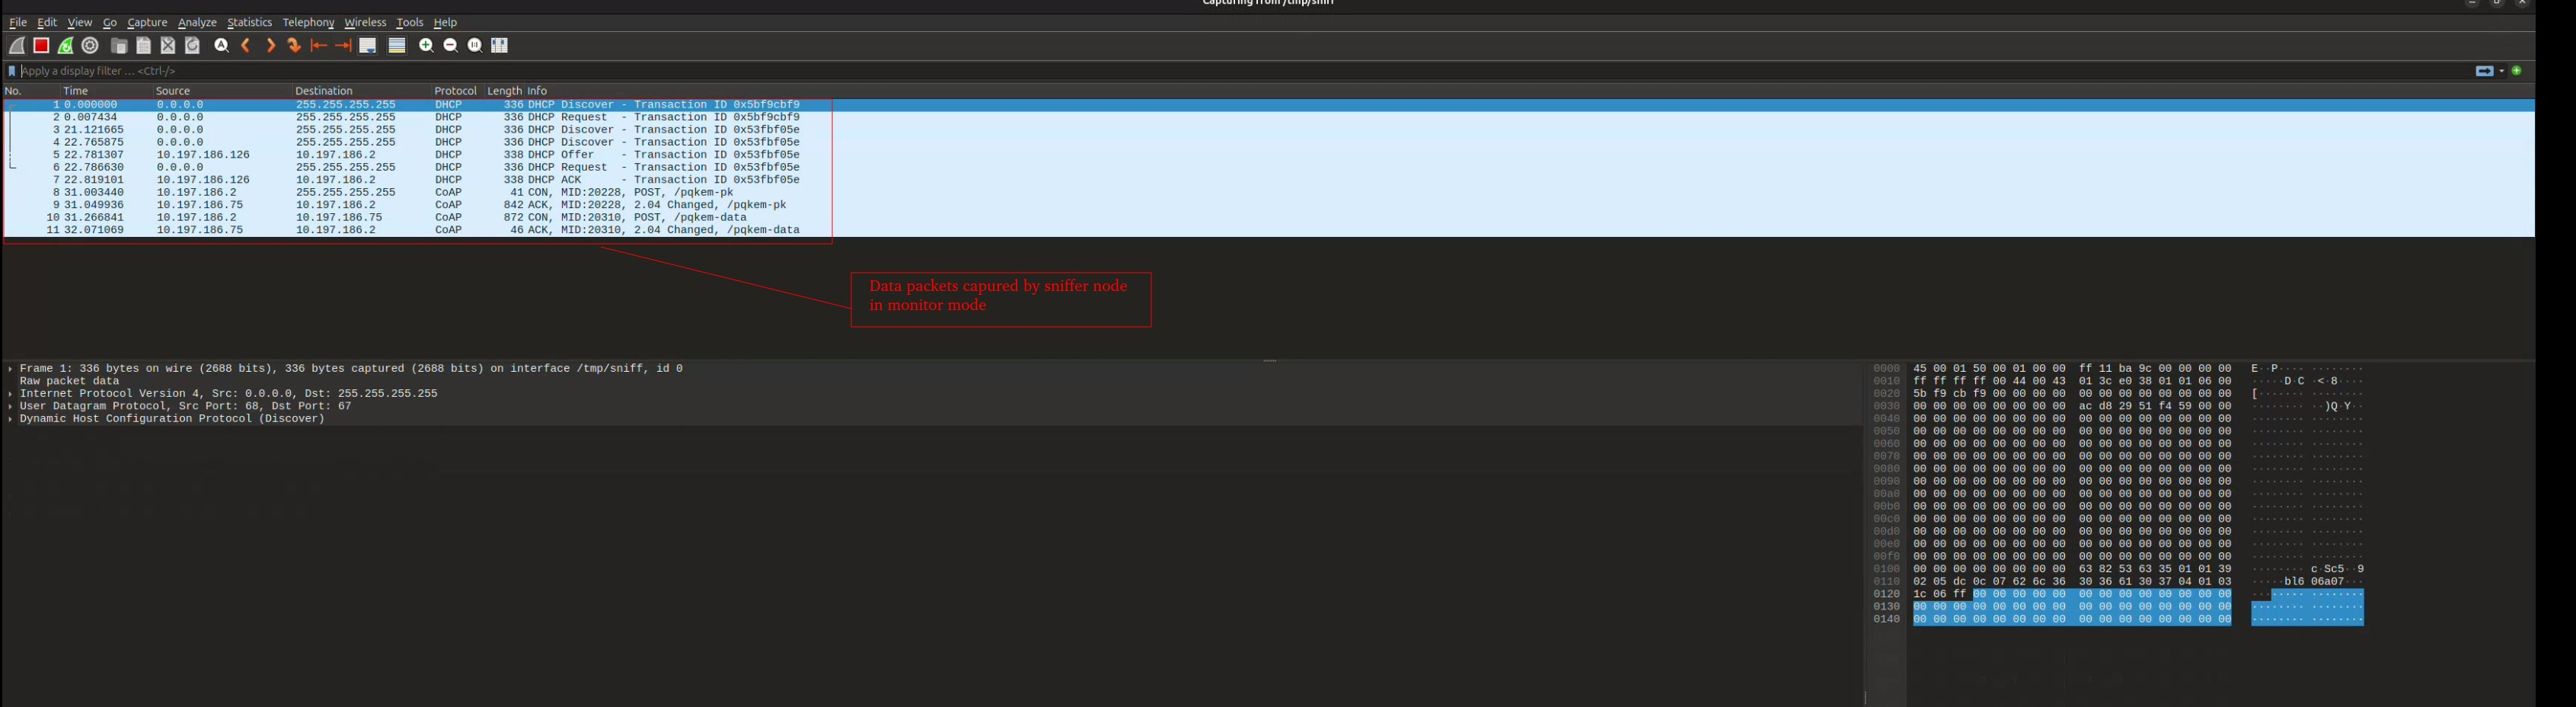
\includegraphics[width=\columnwidth]{data pacekts caputed by sniffer node.jpg.jpeg}
  \caption{Data packets captured by sniffer node – Wireshark (monitor mode)}
  \label{fig:sys-output}
\end{figure}


    \section{limitations}
    The use of ML-KEM-512 as a method for establishing secure keys in post-Quantum computing has been demonstrated through the use of secure data transmission techniques that will work with CoAP/UDP over the BL602 microcontroller. There are several limitations in terms of practical viability for real-world use. First and foremost, while the implementation is a viable proof of concept for key establishment and payload protection, there is no implementation for key rotation and revocation. Furthermore, there is no implementation for key recovery for a compromised device. The practical viability for real-world use in an IoT environment is a concern since these environments tend to have a high duration for the network and the devices. Devices tend to be physical in nature and can be compromised. Hence, key rotation and revocation along with key recovery for a compromised device need to be implemented. The evaluation for the implementation in this project is performed via a single sender and a single gateway. The viability for multiple devices and gateways and network congestion and packet loss scenarios has not been studied. The CoAP protocol operates over UDP. Hence, network congestion and packet loss scenarios tend to be high in an IoT environment. Apart from payload protection via AEAD encryption via AES-CCM, the protocol metadata such as IP and UDP headers and CoAP requests and responses tend to be visible over the network. Hence, an adversary can still get a fair idea of communication patterns. While the implementation demonstrates a high level of protection against sniffing and tampering attacks, the implementation does not address issues related to Denial of Service attacks and packet flooding and Wi-Fi jamming. While the implementation is secure via the use of strong cryptographic primitives and algorithms, these limitations define the boundaries for the implementation and demonstrate a clear direction for future development.

    
    \section{Conclusion and Future work}
    This project has introduced the design and implementation of post-quantum secure system of IoT communication which integrates ML-KEM-512 (Kyber) with an AES-CCM-based authenticated encryption channel atop CoAP over UDP. The prototype demonstrates the existence of post-quantum key establishment being folded into a common IoT stack with a very concrete demonstration that this need not involve redesigning everything. A long-term post-quantum key pair is created on the Gateway side, and stored in on-chip flash and provided as a simple CoAP resource. The Sender can dynamically retrieve this public key at runtime, encapsulate, generate an AEAD key using HKDF and secure application data with AES-CCM all with reasonable latency on a small Wi-Fi microcontroller. A third board which is just a Wi-Fi sniffer combined with a lightweight host script and Wireshark puts a window into the wireless traffic without compromising the underlying cryptographic guarantees. totally, these components constitute a small yet full-fledged platform to do the experimentation of post-quantum key establishment and authenticated encryption under realistic IoT environments.

    This prototype has a number of natural extensions. One thing to start with would be to change the custom payload format to messages that are completely CBOR/COSE-encoded and, in the future, align the design with OSCORE. This would bring the system closer to the standards and simpler to integrate with other CoAP-based IoT stacks. The second direction is to maintain more sets of parameters and algorithms, including ML-KEM-768/1024 or some other NIST-selected KEMs, to investigate the impacts of various security levels on latency, code size and memory on the same hardware. Lastly, a sniffer and capture configuration may become a mini-toolkit, providing some basic anomaly detection or traffic visualization on PQC-protected IoT traffic. This would convert the platform to a reusable environment of both the secure communications and network monitoring experiments.

    
	% Your text goes here, replace blindtext by your text
	
	
	\footnote{\url{https://hs-schmalkalden.de}}
	
	
	
	
	
	\printbibliography[title={References}]

    \begin{table}[H]
\centering
\begin{tabular}{|p{2cm}|p{5cm}|p{2cm}|p{5cm}|}
\hline
\textbf{Reviewer} & \textbf{Review} & \textbf{Decision} & \textbf{Remark} \\
\hline

Reviewer &
AES-CCM is sometimes abbreviated incorrectly as AES-CMM. &
Accepted &
Made corrections.\\
\hline

Reviewer &
The literature review is rather short. The right column on page 3 does not really review literature; instead, it describes the prototype.&
Accepted &
We referred to a few more papers and updated it in the literature review.\\
\hline

Reviewer &
It is specified in three different instances [...] with increased sizes but also increased securities‘. Does this mean key size as well as other
security parameters?&
Accepted &
We confirmed that the terms "size increased" mean large versions of keys/ciphers and Increased Security to Mean Stronger Security.We have also made the clear by stating that ALL VALUES IN BYTES ARE USED , e.g. ML-KEM-512 WILL HAVE A 768 byte Cipher Text; a 32 byte shared secret; an 800 byte public key; and a 1632 byte private key.\\
\hline

Reviewer  &
Cryptographic primitives and operation modes like AES, AEAD, CCM,HKDF and so on are used throughout the text but never
presented/defined.&
Accepted &
Explained in Terminologies\\
\hline

Reviewer &
The font size of Figure 1 is a bit small, making it hard to read.Maybe a UML diagram (like a sequence diagram) would be better suited as well. &
Accepted &
UML diagram is included now. \\
\hline

Reviewer &
Potential attack vectors are not considered: 1. Are
man-in-the-middle-attacks possible? 2. As it appears requests are not limited, DoS attacks seem possible. &
Accepted &
explained in 'Threat model and security testing' and 'Security Analysis and Validation'\\
\hline


\end{tabular}
\label{tab:review}
\end{table}

  \begin{table}[H]
\centering
\begin{tabular}{|p{2cm}|p{5cm}|p{2cm}|p{5cm}|}
\hline
\textbf{Reviewer} & \textbf{Review} & \textbf{Decision} & \textbf{Remark} \\
\hline

Reviewer &
No source code is provided, making it difficult to verify the
results. &
Accepted &
Code is uploaded in Github.\\
\hline

Reviewer &
 Reference 1 has a wrong DOI. Reference 3 contains ‚Ed. By
Albrecht Ude‘ which is also wrong. &
Accepted &
It had been rectified now.\\
\hline

Reviewer &
 unclear whether the public
key is verified in the case of CoAP encryption. If not, this could lead to a man-in-the-middle attack.&
Accepted &
In the existing prototype, the sender gets the gateway public key via CoAP, but it isn't digitally signed or authenticated with certificates or checked for key pinning. As a result, while the project is protected against eavesdropping and tampering , there is no complete protection against a man-in-the-middle attack at the time the public key is first got.\\
\hline

Reviewer &
 the author affiliations are missing and need to be added.&
Accepted &
It has been added now\\
\hline

Reviewer &
the spelling of terms and abbreviations must be consistent throughout the text&
Accepted &
It has been rectified now\\
\hline

Reviewer &
Consistency is also required in the placement of citations &
Accepted &
It has been rectified now\\
\hline

Reviewer &
Grammatical and punctuation mistakes&
Accepted &
It has been rectified now\\
\hline

Reviewer &
splitting Section 5 into two distinct chapters, one
for “Conclusion” and one for “Future Work”, would significantly improve the structure and readability of the text.&
Rejected &
Seperating those will introduce redundancy. \\
\hline

Reviewer &
long-term and session keys are described, the paper does not
discuss key lifecycle management, such as key rotation, key
revocation &
Accepted &
Have mentioned in Limitations \\
\hline


\end{tabular}
\label{tab:review}
\end{table}


 \begin{table}[H]
\centering
\begin{tabular}{|p{2cm}|p{5cm}|p{2cm}|p{5cm}|}
\hline
\textbf{Reviewer} & \textbf{Review} & \textbf{Decision} & \textbf{Remark} \\
\hline

Reviewer &
It does not study multi-device scenarios, network congestion, or packet loss conditions. &
Accepted &
Mentioned in Limitations\\
\hline

Reviewer &
validation is limited to one hardware platform and one post-quantum configuration. &
Accepted &
Mentioned in Limitations\\
\hline

Reviewer &
 does not perform any formal or semi-formal security analysis including discussion of threat models&
Accepted &
explained in 'Threat model and security testing' and 'Security Analysis and Validation' \\
\hline

Reviewer &
 the paper does not provide any comparisons with classical
ECC-based key exchange, other post-quantum key encapsulation
mechanisms, or existing secure IoT frameworks like OSCORE.&
Accepted &
It has been covered in 'Comparison'\\
\hline

Reviewer &
there is a lack of quantitative information regarding the performance and memory usage&
Accepted &
It has been covered in 'Performance Measurements'\\
\hline

Reviewer &
Only ML-KEM-512 was assessed &
Rejected &
In this analysis, we evaluate the smallest parameter set of ML-KEM, which is ML-KEM-512 because it has the best resource requirements for BL602/PineCone platform; hence the results prove that Post-Quantum Key Establishment is feasible with constrained IoT devices.The evaluation of ML-KEM-768 and ML-KEM-1024 remain as future work.\\
\hline

Reviewer &
Redundancy in content&
Accepted &
It has been rectified now\\
\hline




\end{tabular}
\label{tab:review}
\end{table}


\end{document}